\documentclass{beamer}
\usepackage{cmap}
\usepackage[utf8]{inputenc}
\usepackage[russian]{babel}
\usetheme{Antibes}
\usecolortheme{beaver}
\usepackage{graphicx}
\graphicspath{{img/}}

\title{Как и зачем мы делаем Открытый корпус}
\author{В.\,В.~Бочаров\andД.\,В.~Грановский\\\small\it Mathlingvo}
\date{14~мая 2011~г.}
\begin{document}

% title page
\maketitle

%slide 01
\begin{frame}
\frametitle{Жизненный цикл текста}
\begin{enumerate}
\item{Исходный текст}
    \begin{itemize}
    \item{под лицензией, совместимой с CC-BY-SA}
    \item{проходит вычитку}
    \item{делится на абзацы, предложения и токены}
    \end{itemize}
\pause
\item{Морфологические интерпретации}
    \begin{itemize}
    \item{словарь на базе словаря проекта АОТ}
    \item{но морфологический стандарт~--- свой}
    \item{генерируются все возможные гипотезы}
    \end{itemize}
\pause
\item{Полуавтоматика (сейчас её нет)}
    \begin{itemize}
    \item{привязка к словарю на основе эвристик}
    \item{снятие простой неоднозначности}
    \end{itemize}
\pause
\item{Ручное снятие неоднозначности пользователями}
\pause
\item{Разметка доступна для просмотра и скачивания}
\end{enumerate}
\end{frame}

%slide 02
\begin{frame}
\frametitle{Уровни текста}
Концептуальные уровни:
\begin{enumerate}
\item{Графематика}
\item{Морфология}
\item{Синтаксис} (в отдаленных планах)
\item{Семантика} (в совсем отдаленных планах)
\item{Something else?}
\end{enumerate}
\pause
4 иерархических уровня деления (это графематика):
\begin{enumerate}
\item{Текст}
\item{Абзац}
\item{Предложение}
\item{Токен*}
\end{enumerate}
* некоторая последовательность символов без пробелов
\end{frame}

%slide 03
\begin{frame}
\frametitle{Токенизация}
Как разделить текст на эти единицы?
\begin{itemize}
\item{на абзацы~-- взять из источника}
\pause
\item{на предложения~-- пока вручную}
\pause
\item{на токены~-- полуавтоматически}
\end{itemize}
\end{frame}

%slide 03.1
\begin{frame}
\frametitle{Токенизация}
Токенизация должна быть:
\begin{itemize}
\item{единообразной}
\item{удобной для морфологии}
\end{itemize}
Проблемы ручной токенизации:
\begin{itemize}
\item{очень трудоемко}
\item{трудно обеспечить единообразие}
\item{не все отличия видны глазами}
\end{itemize}
\end{frame}

%slide 04
\begin{frame}
\frametitle{Токенизация-2}
Используем простое машинное обучение:
\begin{itemize}
\item{корпус предложений, уже разделенных на токены (внутри текста расставлены границы)}
\pause
\item{набор бинарных характеристических функций (15 шт.)} \\
F1 = <<является ли данный символ пробелом>> \\
... \\
F7 = <<является ли данный символ буквой кириллицы>> \\
... \\
F15 = <<является ли цепочка символов от ближайшего пробела слева до ближайшего пробела справа словарным словом>>
\pause
\item{вычисляем все эти функции для каждой позиции в предложении}
\end{itemize}
\end{frame}

%slide 05
\begin{frame}
\frametitle{Токенизация-3}
Используем простое машинное обучение:
\begin{itemize}
\item{для каждой позиции получается двоичный вектор} \\
Позиция 1: 001000010000000 \\
Позиция 2: 100000100000010 \\
...
\pause
\item{для каждой позиции знаем, проходит ли в ней граница токенов}
\pause
\item{для каждого двоичного вектора на корпусе вычисляется вероятность того, что в позиции с таким вектором есть граница токенов}
\pause
\item{в реальном тексте в каждой позиции тоже вычисляем вектор и смотрим вероятность}
\end{itemize}
\end{frame}

%slide 06
\begin{frame}
\frametitle{Токенизация-4}
Так выглядит обучение:
\begin{figure}
\center{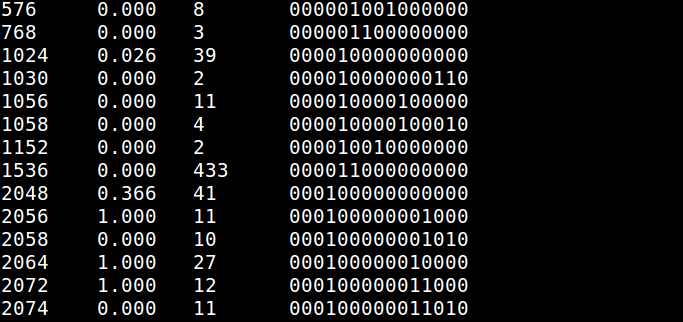
\includegraphics[width=1\linewidth]{2011_nlpseminar_1.png}}
\end{figure}
\end{frame}

%slide 07
\begin{frame}
\frametitle{Токенизация-5}
Получаемое деление~-- вероятностное, поэтому его нужно проверять глазами:
\begin{figure}
\center{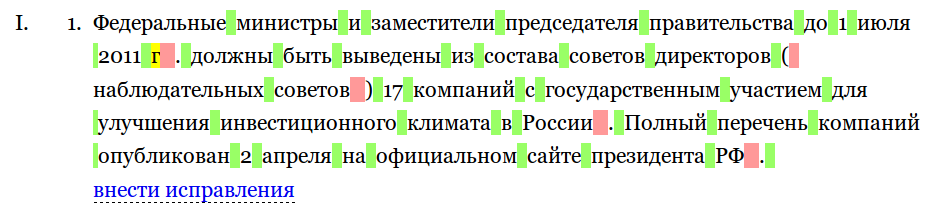
\includegraphics[width=1\linewidth]{2011_nlpseminar_2.png}}
\end{figure}
\pause
\begin{figure}
\center{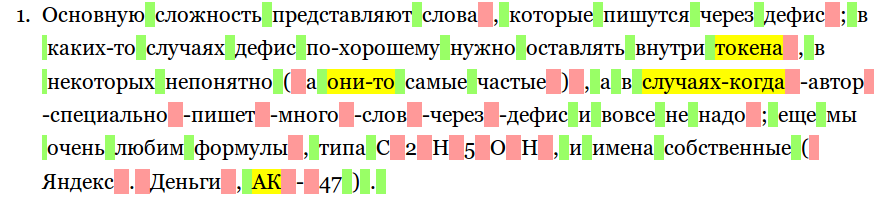
\includegraphics[width=1\linewidth]{2011_nlpseminar_3.png}}
\end{figure}
\end{frame}

%slide 08
\begin{frame}
Вопросы про токенизацию?
\end{frame}

%slide09
\begin{frame}
\frametitle{Морфология}
Суть морфологического уровня:
\begin{itemize}
\item{связать токен с морфологическим словарем}
\item{или обозначить, что токен не является словом}
\end{itemize}
\pause
Зачем нужен морфологический словарь?
\begin{itemize}
\item{можно изменить конкретный разбор конкретной словоформы во всем корпусе сразу}
\item{легче находить опечатки}
\item{в будущем можно будет добавлять лексико-семантическую информацию, почти не меняя разметку}
\end{itemize}
\end{frame}

%slide 10
\begin{frame}
\frametitle{Морфология-2}
\begin{itemize}
\item{за основу взят словарь группы АОТ}
\pause
\item{описание слова = лемма + набор форм (парадигма) + набор граммем леммы}
\pause
\item{описание формы = текст + набор граммем формы}
\pause
\item{леммы связаны между собой связями}
\pause
\item{словарь можно редактировать}
\pause
\item{сочетаемость граммем регулируется моделью морфологии, которая выражена в виде набора правил}
\pause
\item{каждое правило имеет вид: \\
<<Если у [леммы/формы] есть граммема А, то у [леммы/формы] [должна быть/не должно быть/может быть] граммема Б>>}
\end{itemize}
\end{frame}

%slide 11
\begin{frame}
\frametitle{Морфология-3}
Модель нужна, чтобы отслеживать ошибки, присутствующие в словаре изначально или вносимые редакторами. \\
Примеры правил:
\begin{itemize}
\item{NOUN -> NMbr (лемма -> форма, обязательно)}
\item{VERB -> ASpc (лемма -> лемма, обязательно)}
\item{indc -> TEns (форма -> форма, обязательно)}
\item{VERB -> Impe (лемма -> лемма, возможно)}
\item{Impe -> PErs (лемма -> форма, запрещено)}
\end{itemize}
Всего сейчас 107 граммем и 127 правил + 218 автоматически выведенных.
\end{frame}

%slide 12
\begin{frame}
\frametitle{Морфология-4}
Итого в словаре бывает 5 типов ошибок:
\begin{enumerate}
\item{неизвестная граммема}
\item{несовместимые граммемы}
\item{явно не разрешенная правилами граммема}
\item{отсутствует обязательная граммема}
\item{две формы в рамках парадигмы имеют полностью совпадающие наборы граммем}
\end{enumerate}
\end{frame}

%slide 13
\begin{frame}
Вопросы про морфологию?
\end{frame}

%slide 14
\begin{frame}
\frametitle{Разрешение неоднозначности}
2 этапа: (полу)автоматический (сейчас нет), ручной.
\pause

Ручное разрешение морфологической неоднозначности~-- основная задача, для которой мы хотим привлекать пользователей-разметчиков.
\pause

От разметчика требуется:
\begin{itemize}
\item{исключить неверные разборы, в идеальном случае~-- выбрать один}
\item{или отметить, что верный разбор отсутствует}
\end{itemize}
\end{frame}

%slide 15
\begin{frame}
\frametitle{Интерфейс разрешения неоднозначности}
(Here be live demonstration)
\end{frame}

%slide 16
\begin{frame}
\frametitle{Contacts}
\begin{center}
Берем студентов на практику!\\[\bigskipamount]
\LARGE http://opencorpora.org\\[\bigskipamount]
\Large\texttt{granovsky@opencorpora.org\\bocharov@opencorpora.org}
\end{center}
\end{frame}

\end{document}
